\section{Using Qt framework}
Basic Qt library structure is known to us but we need to know something about Qt-related development evnironments and tools. You can develop Qt applications in any text editor or in major development environment, including Microsoft Visual Studio{Visual Studio}. Some tools are part of Qt framework, however. This includes young and thriving Qt Creator\index{Qt Creator} development environment.

Every Qt/\cpp programmmer should be aware of existence of certain rules concerning source code appearance. These rules are called \textit{conventions}\index{convention} and you will learn about them too.

\subsection{Qt Creator}
Qt Creator (see \autoref{figure:qtcreator}) is fully-featured \cpp \& JavaScript development environment. It is suitable for plain \cpp development as well as for Qt development. Qt Creator is part of Qt SDK, thus can be installed along with Qt libraries.

\begin{figure}[ht]
\centering
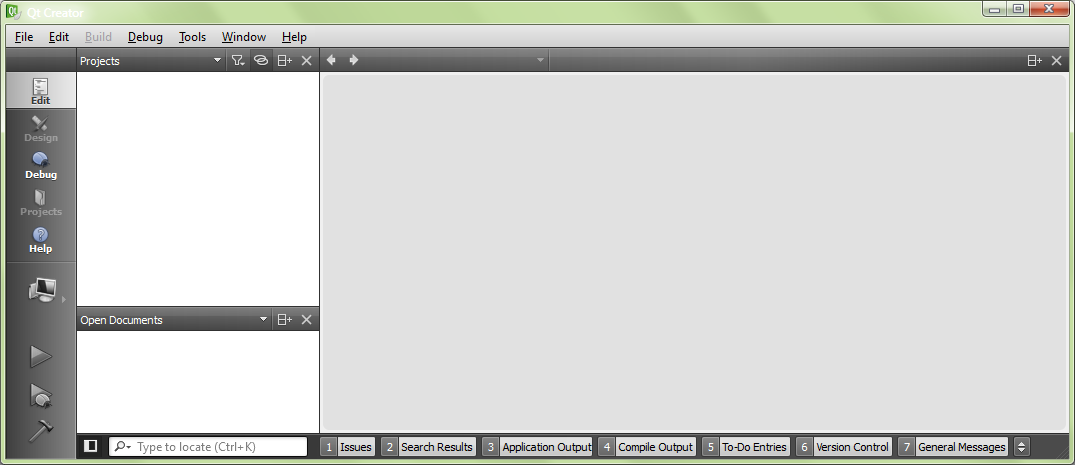
\includegraphics[width=14.5cm]{graphics/laboratory/03-qtcreator.png}
\caption{Qt Creator empty environment}\label{figure:qtcreator}
\end{figure}

Qt Creator supports big collection of features:
\begin{itemize}
\item multiple build systems (CMake\index{CMake}, Autotools\index{Autotools} and QMake\index{QMake})
\item syntax highlighting for more than one hundred programming languages
\item auto-completion for variables, functions and macros (see \autoref{figure:qtcreatorauto})
\item consistent look on every supported operating system
\item many plugins
\item refactoring facilities
\item tools for debugging
\item cooperation with Android SDK
\item dynamic keyboard shortcuts
\item integrated Qt help system (see \autoref{figure:qtcreatorhelpfull})
\item context-aware help (see \autoref{figure:qtcreatorhelp})
\item support for simultaneously installed Qt frameworks
\item integrated Qt Designer for \fdocabbrevref{GUI} design
\item sharing source code via online services
\item many more\ldots
\end{itemize}

\begin{figure}[ht]
\centering
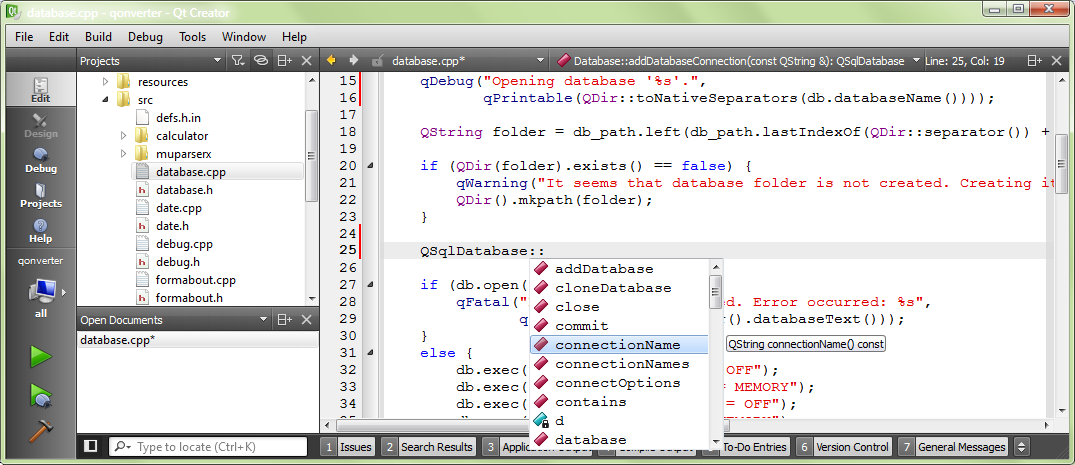
\includegraphics[width=14.5cm]{graphics/laboratory/04-qtcreator-auto.png}
\caption{Qt Creator auto-completion}\label{figure:qtcreatorauto}
\end{figure}

\begin{figure}[ht]
\centering
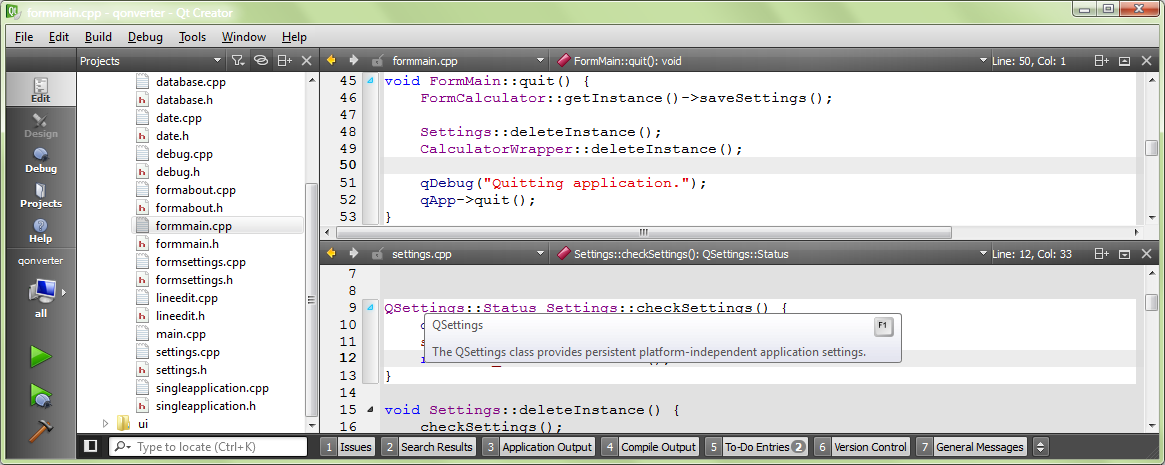
\includegraphics[width=14.5cm]{graphics/laboratory/05-qtcreator-help.png}
\caption{Qt Creator context-aware help}\label{figure:qtcreatorhelp}
\end{figure}

\begin{figure}[ht]
\centering
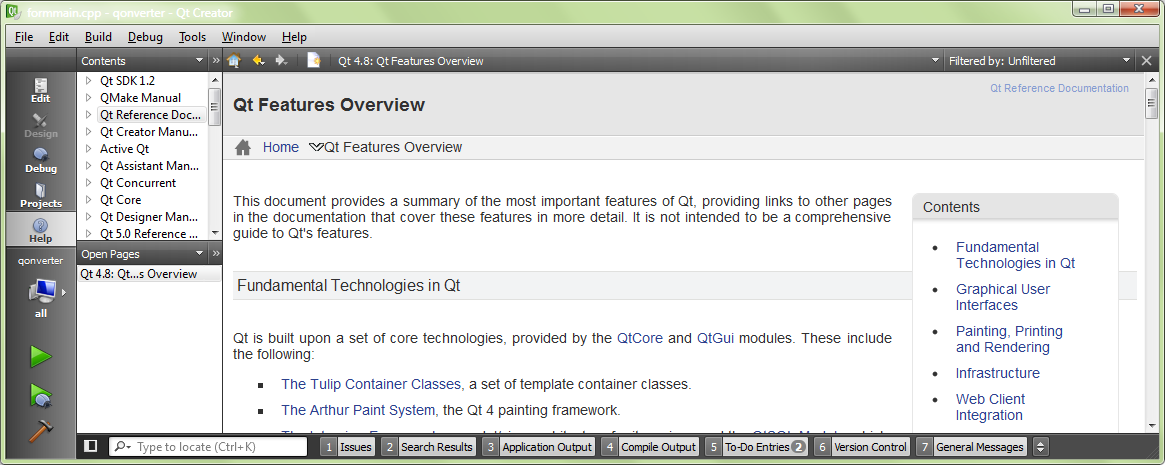
\includegraphics[width=14.5cm]{graphics/laboratory/06-qtcreator-help-full.png}
\caption{Qt Creator full reference documentation}\label{figure:qtcreatorhelpfull}
\end{figure}

\subsection{Qt Designer}
Qt Designer\index{Qt Designer} (see \autoref{figure:designer}) is a tool for user interface design. It is standalone application which is integrated into Qt Creator too.

\begin{figure}[ht]
\centering
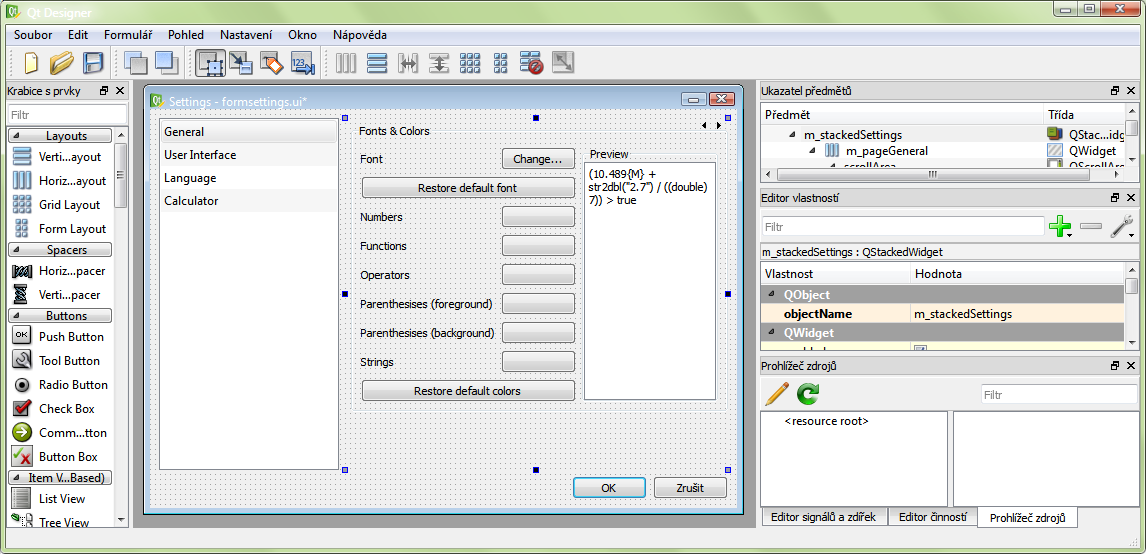
\includegraphics[width=14.5cm]{graphics/laboratory/07-designer.png}
\caption{Qt Designer environment}\label{figure:designer}
\end{figure}

\subsection{Tools and chains}

\subsection{Conventions}
% vkladani hlavickovych souboru, nazvy promennych atp